\subsection{Kavicsos talajon helyben forgás}
A \ref{fig:Left_n50Right50a} megfigyelhető amint a robot kavicsos talajon differenciálisan fordul 60 másodpercen keresztül, ezalatt háromszor teljen korbefordul. A palyat tekintve letrejon egy oldaliranyu mozgás is igy az X tengelyen 0.22m es a Y tengelyen 0.6m mozdul el. Az oldaliranyu mozgas a nem egyenlo surlodasi erok miatt jon letre.
A fordulas kozben a kerekek kovetik az eloirt referencia szogsebesegeket, amint az \ref{fig:Left_n50Right50x} abran is lathato.
A frdulasi szogsebeseg 20 \degree/s, az X es Y tengelyen valo sebesseg elhanyagolhato nagysagu de jelen van mivel a robot forgasi kozepontja elmozdul \ref{fig:Left_n50Right50b}.

\renewcommand{\nth}{2}
\renewcommand{\GlobalPath}{Meresek/Mozgasok/NormalMukodes/DiferencialisanHelybeKavicsos/}
\renewcommand{\secondImage}{*}



\begin{figure}[H]
  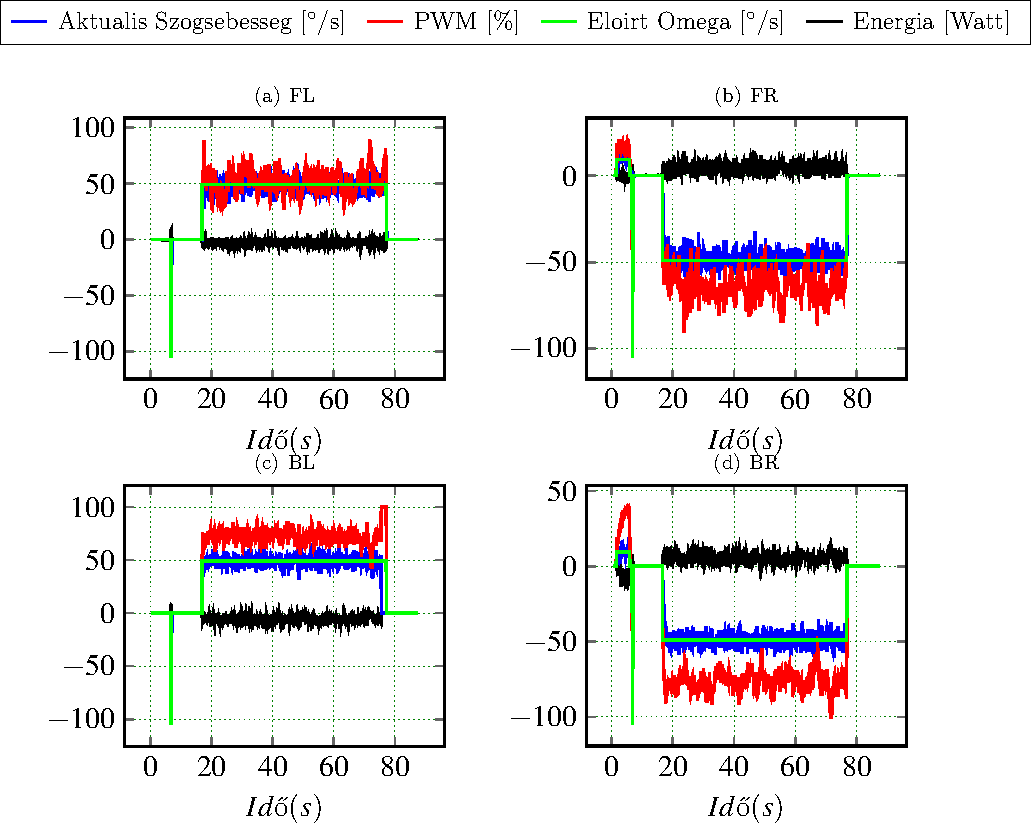
\includegraphics{tikz/Left_n50Right50x.pdf}
  \caption{$SSMR-4W$ típusú robot mozgása, tengelyekre bontva, kereksebessegek BL=FL=0 es a FR=BR= 50\degree/s}
  \label{fig:Left_n50Right50x}
\end{figure}


\begin{figure}[H]
  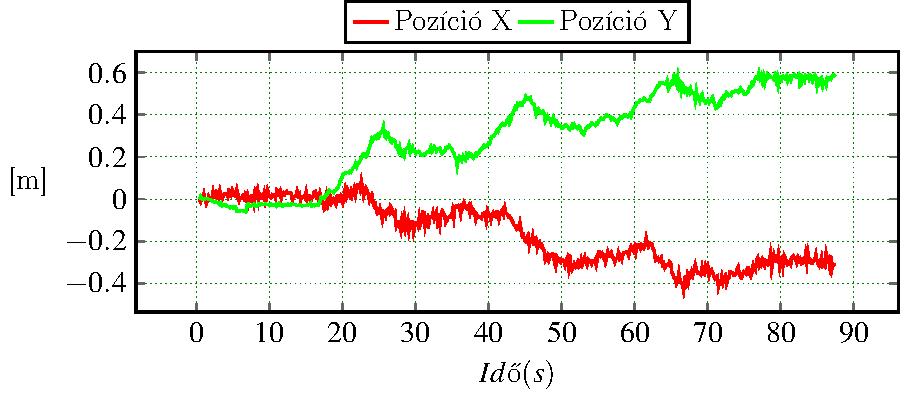
\includegraphics{tikz/Left_n50Right50a.pdf}
  \caption{$SSMR-4W$ típusú robot mozgása, tengelyekre bontva, kereksebessegek BL=FL=-50 es a FR=BR= 50\degree/s}
  \label{fig:Left_n50Right50a}
\end{figure}


\begin{figure}[H]
  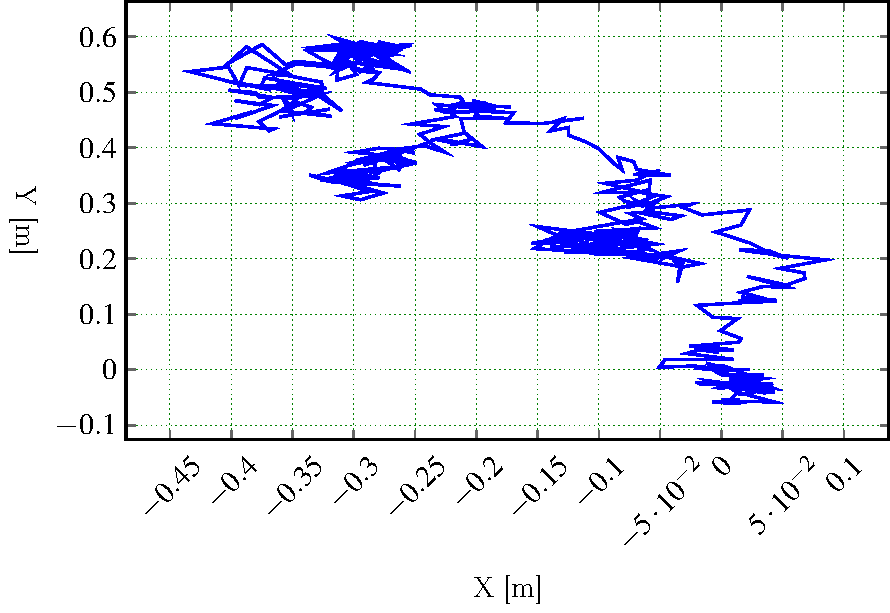
\includegraphics{tikz/Left_n50Right50b.pdf}
  \caption{$SSMR-4W$ típusú robot altal leirt palya, kereksebessegek BL=FL=-50 es a FR=BR= 50\degree/s}
    \label{fig:Left_n50Right50b}
\end{figure}



\begin{figure}[H]
  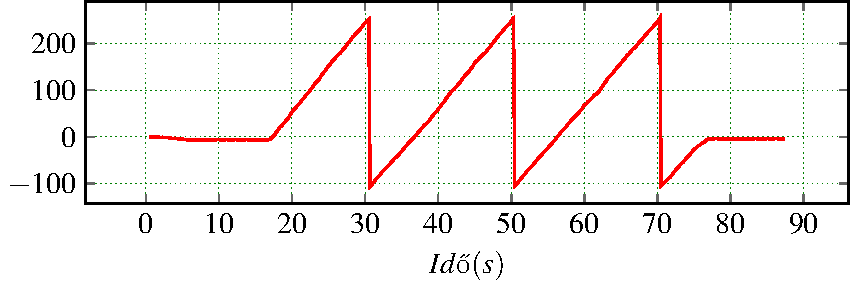
\includegraphics{tikz/Left_n50Right50c.pdf}
  \caption{$SSMR-4W$ típusú robot orientacioja, kereksebessegek BL=FL=-50 es a FR=BR= 50\degree/s}
    \label{fig:Left_n50Right50c}
\end{figure}


\begin{figure}[H]
  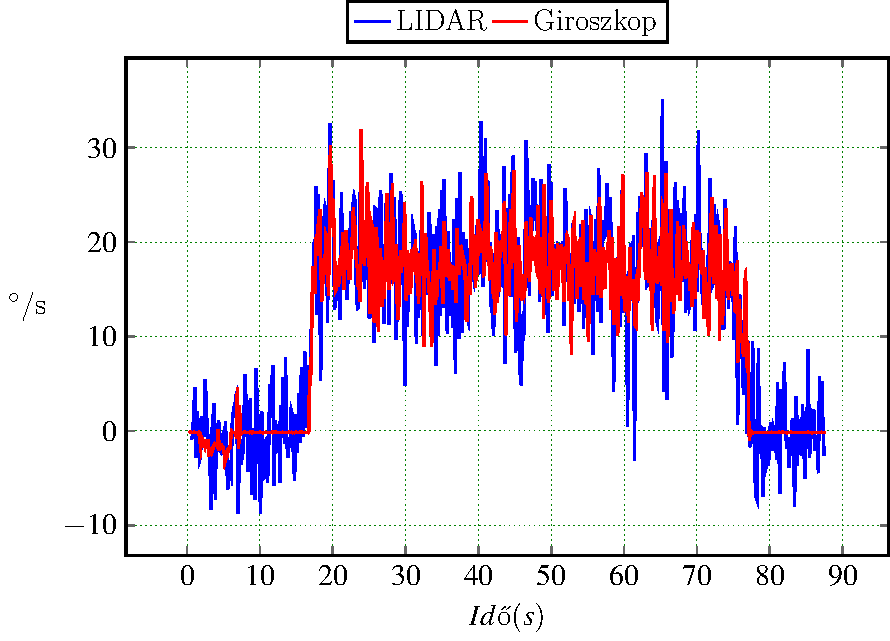
\includegraphics{tikz/Left_n50Right50d.pdf}
  \caption{$SSMR-4W$ típusú robot fordulasi szogsebessege, kereksebessegek BL=FL=-50 es a FR=BR= 50\degree/s}
    \label{fig:Left_n50Right50d}
\end{figure}









